% Cruise Range Chart - Wheel Pants OFF
\begin{figure}[t]
% \addcontentsline{toc}{section}{Figure \ref{Cruise-range} Cruise Range}
\addcontentsline{toc}{section}{CRUISE RANGE - WHEEL PANTS OFF}
\begin{center}
\begin{perfhdr}CRUISE RANGE - WHEEL PANTS OFF\\
\end{perfhdr}

\begin{minipage}{5in}
  \begin{flushleft}
    CONDITIONS:\\
    Wheel Pants OFF, Gear Leg Fairings ON\\
    43 USG Usable Fuel.\\
    Standard atmosphere.\\
    No wind.\\
    Includes 1.0 USG fuel for start, taxi and takeoff and 8 USG or 45 mn reserve.\\
    Climb at full power and best climb speed as defined on the Maximum Climb Chart\\
    Lean during climb for best power.\\
    Cruise with mixture set to best power for 75\% power.  \\
    Cruise with mixture set to 50\textdegree F lean of peak EGT for 65\% power or less, except mixture set to best power if more than 2600 rpm required with mixture set lean of peak EGT.\\
    Descend at cruise TAS at 6 nm per 1000 ft.\\
    \end{flushleft}
\end{minipage}\\
\vspace{5ex}
% GNUPLOT: LaTeX picture with Postscript
\begingroup
  \makeatletter
  \providecommand\color[2][]{%
    \GenericError{(gnuplot) \space\space\space\@spaces}{%
      Package color not loaded in conjunction with
      terminal option `colourtext'%
    }{See the gnuplot documentation for explanation.%
    }{Either use 'blacktext' in gnuplot or load the package
      color.sty in LaTeX.}%
    \renewcommand\color[2][]{}%
  }%
  \providecommand\includegraphics[2][]{%
    \GenericError{(gnuplot) \space\space\space\@spaces}{%
      Package graphicx or graphics not loaded%
    }{See the gnuplot documentation for explanation.%
    }{The gnuplot epslatex terminal needs graphicx.sty or graphics.sty.}%
    \renewcommand\includegraphics[2][]{}%
  }%
  \providecommand\rotatebox[2]{#2}%
  \@ifundefined{ifGPcolor}{%
    \newif\ifGPcolor
    \GPcolorfalse
  }{}%
  \@ifundefined{ifGPblacktext}{%
    \newif\ifGPblacktext
    \GPblacktexttrue
  }{}%
  % define a \g@addto@macro without @ in the name:
  \let\gplgaddtomacro\g@addto@macro
  % define empty templates for all commands taking text:
  \gdef\gplbacktext{}%
  \gdef\gplfronttext{}%
  \makeatother
  \ifGPblacktext
    % no textcolor at all
    \def\colorrgb#1{}%
    \def\colorgray#1{}%
  \else
    % gray or color?
    \ifGPcolor
      \def\colorrgb#1{\color[rgb]{#1}}%
      \def\colorgray#1{\color[gray]{#1}}%
      \expandafter\def\csname LTw\endcsname{\color{white}}%
      \expandafter\def\csname LTb\endcsname{\color{black}}%
      \expandafter\def\csname LTa\endcsname{\color{black}}%
      \expandafter\def\csname LT0\endcsname{\color[rgb]{1,0,0}}%
      \expandafter\def\csname LT1\endcsname{\color[rgb]{0,1,0}}%
      \expandafter\def\csname LT2\endcsname{\color[rgb]{0,0,1}}%
      \expandafter\def\csname LT3\endcsname{\color[rgb]{1,0,1}}%
      \expandafter\def\csname LT4\endcsname{\color[rgb]{0,1,1}}%
      \expandafter\def\csname LT5\endcsname{\color[rgb]{1,1,0}}%
      \expandafter\def\csname LT6\endcsname{\color[rgb]{0,0,0}}%
      \expandafter\def\csname LT7\endcsname{\color[rgb]{1,0.3,0}}%
      \expandafter\def\csname LT8\endcsname{\color[rgb]{0.5,0.5,0.5}}%
    \else
      % gray
      \def\colorrgb#1{\color{black}}%
      \def\colorgray#1{\color[gray]{#1}}%
      \expandafter\def\csname LTw\endcsname{\color{white}}%
      \expandafter\def\csname LTb\endcsname{\color{black}}%
      \expandafter\def\csname LTa\endcsname{\color{black}}%
      \expandafter\def\csname LT0\endcsname{\color{black}}%
      \expandafter\def\csname LT1\endcsname{\color{black}}%
      \expandafter\def\csname LT2\endcsname{\color{black}}%
      \expandafter\def\csname LT3\endcsname{\color{black}}%
      \expandafter\def\csname LT4\endcsname{\color{black}}%
      \expandafter\def\csname LT5\endcsname{\color{black}}%
      \expandafter\def\csname LT6\endcsname{\color{black}}%
      \expandafter\def\csname LT7\endcsname{\color{black}}%
      \expandafter\def\csname LT8\endcsname{\color{black}}%
    \fi
  \fi
  \setlength{\unitlength}{0.0500bp}%
  \begin{picture}(7200.00,5040.00)%
    \gplgaddtomacro\gplbacktext{%
      \csname LTb\endcsname%
      \put(1210,704){\makebox(0,0)[r]{\strut{}0}}%
      \csname LTb\endcsname%
      \put(1210,1722){\makebox(0,0)[r]{\strut{}5,000}}%
      \csname LTb\endcsname%
      \put(1210,2740){\makebox(0,0)[r]{\strut{}10,000}}%
      \csname LTb\endcsname%
      \put(1210,3757){\makebox(0,0)[r]{\strut{}15,000}}%
      \csname LTb\endcsname%
      \put(1210,4775){\makebox(0,0)[r]{\strut{}20,000}}%
      \csname LTb\endcsname%
      \put(1342,484){\makebox(0,0){\strut{} 450}}%
      \csname LTb\endcsname%
      \put(1949,484){\makebox(0,0){\strut{} 500}}%
      \csname LTb\endcsname%
      \put(2556,484){\makebox(0,0){\strut{} 550}}%
      \csname LTb\endcsname%
      \put(3162,484){\makebox(0,0){\strut{} 600}}%
      \csname LTb\endcsname%
      \put(3769,484){\makebox(0,0){\strut{} 650}}%
      \csname LTb\endcsname%
      \put(4376,484){\makebox(0,0){\strut{} 700}}%
      \csname LTb\endcsname%
      \put(4983,484){\makebox(0,0){\strut{} 750}}%
      \csname LTb\endcsname%
      \put(5589,484){\makebox(0,0){\strut{} 800}}%
      \csname LTb\endcsname%
      \put(6196,484){\makebox(0,0){\strut{} 850}}%
      \csname LTb\endcsname%
      \put(6803,484){\makebox(0,0){\strut{} 900}}%
      \put(176,2739){\rotatebox{-270}{\makebox(0,0){\strut{}Altitude (ft)}}}%
      \put(4072,154){\makebox(0,0){\strut{}Cruise Range - Wheel Pants OFF (NM)}}%
      \put(1762,1009){\rotatebox{83}{\makebox(0,0)[l]{\strut{}75\% Power}}}%
      \put(3512,1213){\rotatebox{88}{\makebox(0,0)[l]{\strut{}65\% Power}}}%
      \put(4265,1213){\rotatebox{73}{\makebox(0,0)[l]{\strut{}55\% Power}}}%
      \put(5036,1213){\rotatebox{71}{\makebox(0,0)[l]{\strut{}45\% Power}}}%
      \put(5700,1213){\rotatebox{71}{\makebox(0,0)[l]{\strut{}35\% Power}}}%
    }%
    \gplgaddtomacro\gplfronttext{%
    }%
    \gplbacktext
    \put(0,0){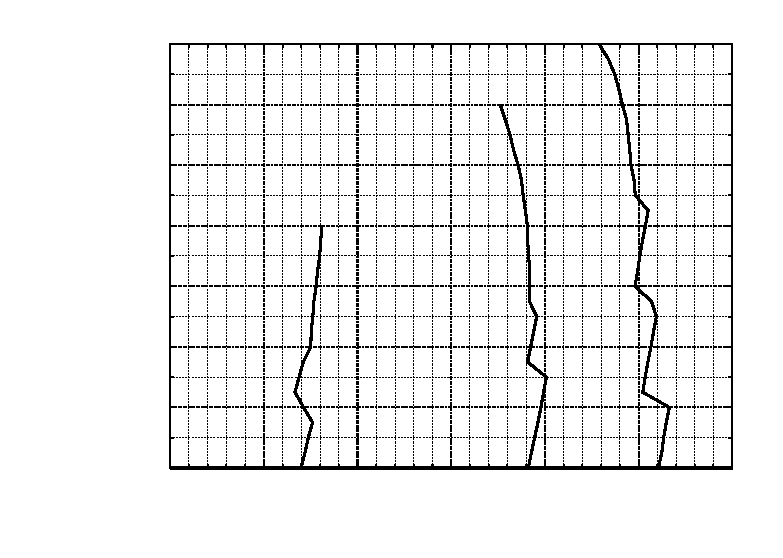
\includegraphics{../graphs/cruise_range_wheel_pants_off}}%
    \gplfronttext
  \end{picture}%
\endgroup
\end{center}  % for gnuplot epslatex, latex or pslatex mode
\caption{Cruise Range - Wheel Pants OFF}
\label{Cruise-range-WP-OFF}
\end{figure}
\clearpage


